\begin{figure}[htbp]\centering
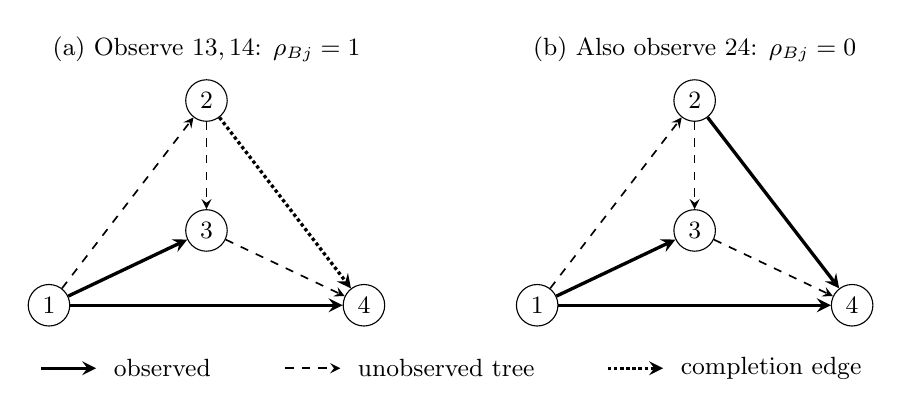
\begin{tikzpicture}[>=stealth,
  vertex/.style={circle,draw,fill=white,inner sep=2pt,minimum size=15pt},
  observed/.style={->,line width=1.2pt},
  forest/.style={->,dashed,line width=.6pt},
  completion/.style={->,densely dotted,line width=1.2pt},
  every node/.style={font=\small}]
\foreach \panel/\shift in {a/0,b/6.2}{
  \begin{scope}[xshift=\shift cm]
    \node[vertex] (\panel1) at (0,0) {$1$};
    \node[vertex] (\panel2) at (2,2.6) {$2$};
    \node[vertex] (\panel3) at (2,.95) {$3$};
    \node[vertex] (\panel4) at (4,0) {$4$};
    \draw[observed] (\panel1) -- (\panel3);
    \draw[observed] (\panel1) -- (\panel4);
    \draw[forest] (\panel1) -- (\panel2);
    \draw[forest] (\panel2) -- (\panel3);
    \draw[forest] (\panel3) -- (\panel4);
  \end{scope}
}
\draw[completion] (a2) -- (a4);
\draw[observed] (b2) -- (b4);
\node at (2,3.25) {(a) Observe $13,14$: $\rho_{Bj}=1$};
\node at (8.2,3.25) {(b) Also observe $24$: $\rho_{Bj}=0$};
\draw[observed] (-.1,-.8) -- (.6,-.8);
\node[anchor=west] at (.7,-.8) {observed};
\draw[forest] (3,-.8) -- (3.7,-.8);
\node[anchor=west] at (3.8,-.8) {unobserved tree};
\draw[completion] (7.1,-.8) -- (7.8,-.8);
\node[anchor=west] at (7.9,-.8) {completion edge};
\end{tikzpicture}
\caption{Individual-product completion on one $K_4$ block $B$ for a fixed
label $j$. All arcs point from the smaller vertex to the larger one.
In (a), the unobserved edges $12,23,24,34$ have one independent cycle;
the spanning tree $12,23,34$ leaves $24$ as the single completion edge.
Observing $24$ gives (b), the forest complement in \cref{ex:forest-k4},
so no additional coordinate is needed for this block--label pair.}
\label{fig:observation-completion}
\end{figure}
